\section{Network Architecture}\label{design:comPiEv3}
In \autoref{sec:design-avSystemArchitecture} an overall system architecture was described, this section will describe in more detail the architecture of the network that allows for the communication between the PC, Raspberry Pi and the EV3.
As the vehicle will use more than one device when running, it will need a way to connect its devices.
Each device has its own individual responsibilities, the EV3 controls the motors on the vehicle and the Pi is responsible for calculating the steering angle based on the input from the camera. 
Additionally, a PC will be used for communicating with the vehicle, in order to manually steer the vehicle during the Data Collection phase, as mentioned in \autoref{sec:design-avSystemArchitecture}.

Because they each have individual responsibilities they need a way to communicate.
In order for the EV3 to control the steering motor of the vehicle correctly, it requires the angle from the Pi.
Without it, the vehicle wouldn't be capable of driving along the road. 

There are two ways of establishing a line of communication between the two devices: Wired or Wireless

%Wired: 
Connecting the devices through a wired connection, would involve a physical cable running between the devices. 
There exists a number of different ways to do this, like Ethernet, USB, I2C and more. 
Wired connections tend to have faster and more stable connection than it's wireless counterparts. 

%Wireless: 
Connecting the devices wirelessly, would involve connecting them through another network like WiFi or directly through Bluetooth.
This would avoid a cable between the devices and would mean they weren't physically connected.
This, in turn, would put less limitations on the distance between the devices and make them more portable.  

Due to the proximity of the EV3 and Pi, as well as the fact that both devices will be mounted directly on the vehicle, a wired connection will be used for connecting the devices. Since performance is prefered over portability, it has been decided to use a wired connection.

While a wireless connection wasn't useful when connecting the EV3 and Pi, it is when connecting the PC to the Pi.
As the PC won't be mounted on the vehicle, having cables between the vehicle and the PC could potentially cause problems while driving. 
Because of this, the PC will be connected wirelessly to the Pi. 

\begin{figure} [H]
    \centering
    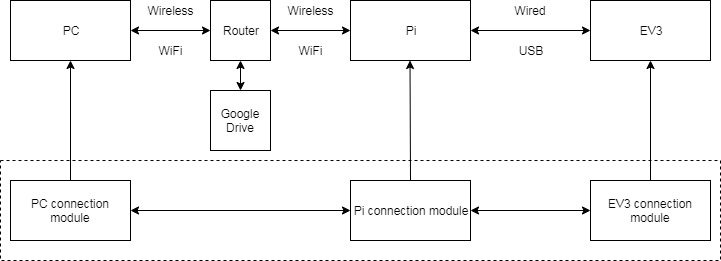
\includegraphics[width=\textwidth]{images/design/Pc_Pi_EV3_Connection.jpg}
    \caption{Diagram of the network architecture}
    \label{fig:PC_Pi_EV3_com}
\end{figure}

As seen in \autoref{fig:PC_Pi_EV3_com}, the PC will connect wirelessly to the Pi through a router and the Pi and EV3 are connected through USB. 
The purpose of connecting the Pi to the router is to make it more convenient to upload data to Google Drive, download new trained models from Google Drive, as well as updating code on the Pi from the Github repository. 
Any communication between the PC and the EV3 will happen through the Pi. 
So when the PC sends a command that has to go to the EV3, the Pi is responsible for forwarding the command. 
Each device will have a connection module, as seen in the dotted box. 
These modules are responsible for all the communication happening between the devices.